\section{问题四模型建立与求解}
\label{sec:question4}

\subsection{问题四分析}

问题四将已知分时电价改为随时间变化的交易电价，并要求分别推广问题二的日前采购和问题三的滚动策略。此时采购数量不仅受净负荷预测影响，还取决于缺口出现时的价格：同样少买1 kWh，若恰逢高价，五倍紧急补购造成的损失更大。因此，将负荷误差与价格误差分别独立抽样，可能破坏与费用直接相关的联合结构。

本问保留电池的状态方程、容量与功率限制，以及问题三已经确定的结算口径，改变外层的不确定输入和相应经济系数。附件4给出的实际价格用于逐时结算，未来尚未揭示的实际价格不能进入日前或滚动决策。先用价格加权分位数解释联合建模的原因，再以同日残差构造价荷场景；日前版保留母模型，滚动版沿用第\ref{sec:q3_candidate_screening}节的全时点候选筛选，最终比较两种可执行策略的实际费用。两案的预测配置、候选筛选设置与一月形成的初态不同，横向差异只作整体策略比较，不能全归因于单一模块。

\subsection{问题四模型建立}

\subsubsection{价格与需求相关时的采购分位数}

先考虑无储能单时段子问题。设未来净需求$X$与未来结算电价$P$可能相关，日前在已有信息下固定$q\ge0$；假设$P>0$几乎处处成立、$0<\mathbb E[P]<\infty$、$\mathbb E[PX_+]<\infty$，且富余购电无残值。期望费用为
\begin{equation}
 J_4(q)=\mathbb E[P]q+5\mathbb E[P(X-q)_+],\qquad q\ge0.
 \label{eq:mech_q4_cost}
\end{equation}
若将价格直接用均值替代，通常会遗漏$P$与缺口$(X-q)_+$的关联。为保留这一作用，定义
\begin{equation}
 G(x)=\frac{\mathbb E[P\,\mathbf 1_{\{X\le x\}}]}{\mathbb E[P]},\qquad
 G(x^-)=\frac{\mathbb E[P\,\mathbf 1_{\{X<x\}}]}{\mathbb E[P]}.
 \label{eq:mech_weighted_cdf}
\end{equation}
正价与有限期望保证$G$是合法分布函数。式\eqref{eq:mech_q4_cost}为凸函数，其次梯度为
\begin{equation}
 \partial J_4(q)=\mathbb E[P][5G(q^-)-4,\ 5G(q)-4].
 \label{eq:mech_q4_subgradient}
\end{equation}
内点最优条件为$G(q^-)\le0.8\le G(q)$，若最优点处连续，则
$\mathbb E[P\mathbf 1_{\{X\le q\}}]/\mathbb E[P]=0.8$。结合非负约束，可取
\begin{equation}
 q_4^\star=\max\{0,G^{-1}(0.8)\}.
 \label{eq:mech_weighted_quantile}
\end{equation}
对于离散场景$(x_s,p_s,\pi_s)$，只需把概率改写为
\begin{equation}
 \widetilde\pi_s=\frac{\pi_sp_s}{\sum_j\pi_jp_j},\qquad
 G(x)=\sum_{s:x_s\le x}\widetilde\pi_s.
 \label{eq:mech_scenario_reweight}
\end{equation}
于是最优采购对应价格加权的需求80\%分位数。若价荷独立，$G=F_X$，退化为问题二的普通分位数；若高需求更常伴随高价，该类场景的经济权重上升。该推导解释为何要保留联合关系，但只适用于无储能单时段。完整模型中的容量、效率、功率及跨时段能量价值，仍须由联合优化处理。

\subsubsection{合法价格预测与同日价荷残差场景}

以问题二、三已经选定的负荷和光伏预测配置为基础，只在1月验证期比较候选价格预测器，再冻结用于2--12月。动态日前案采用最近四个同星期日价格均值；动态滚动案采用最近两个同星期日均值。日前案负荷为最近两个同星期日均值、光伏为近三日均值；滚动案使用附件发布的光伏预报，并保留问题三的负荷偏差反馈。

动态滚动案在$\tau>0$时对价格采用与式\eqref{eq:q3_load_bias}、\eqref{eq:q3_load_update}相同的因果偏差修正：用此前12段实际价格相对零时预测的均值偏差，按六小时尺度衰减，并限制在零时预测的$\pm30\%$；价格预测正值下界取$10^{-6}$元/kWh。这些计算仅使用已经观察到的价格，不读取当天剩余实际价格。

对过去完整日$j<D$，分别求同发布时间的净负荷残差$\epsilon^n_{j,t}$和价格残差
\begin{equation}
 \epsilon^p_{j,t}=p_{j,t}-\widehat p^{(\tau)}_{j,t},\qquad t\ge\tau.
 \label{eq:q4_price_residual}
\end{equation}
两类残差按同一历史日配对，构成
\begin{equation}
 n_{t,s}=\widehat n_t+\epsilon^n_{j_s,t},\qquad
 p_{t,s}=\max\{0.01,\widehat p_t+\epsilon^p_{j_s,t}\}.
 \label{eq:joint_scenario}
\end{equation}
历史窗口至多28日，主案完整保留、等权赋值；价荷不拆日、不逐点重排。这样同时保存日内连续误差和价荷联系。若在12场景对照中进行代表日压缩，则先分别标准化净负荷与价格残差块再计算轨迹距离，防止不同单位的数值尺度支配选择。

式\eqref{eq:joint_scenario}的0.01元/kWh仅是外层加性场景的正价下界，并未改写实际价格序列。原始最低价0.0076元/kWh仍用于实际账单；实际结算价、合法点预测及合成场景价是三个不同对象。图\ref{fig:q4-correlation}在策略冻结后，对2--12月48096个时段的负荷、光伏、净负荷与电价作描述性Pearson相关分析。净负荷与价格的实际值相关系数为0.2620，按当时合法预测计算的残差相关系数为0.3468，显示分开两类残差会改变样本中的联合关系。该图不参与一月选型或未来场景构造，不授权提前使用评价期真值；未作时序依赖校正或显著性推断，相关系数也不表示因果效应。

\begin{figure}[htbp]\centering
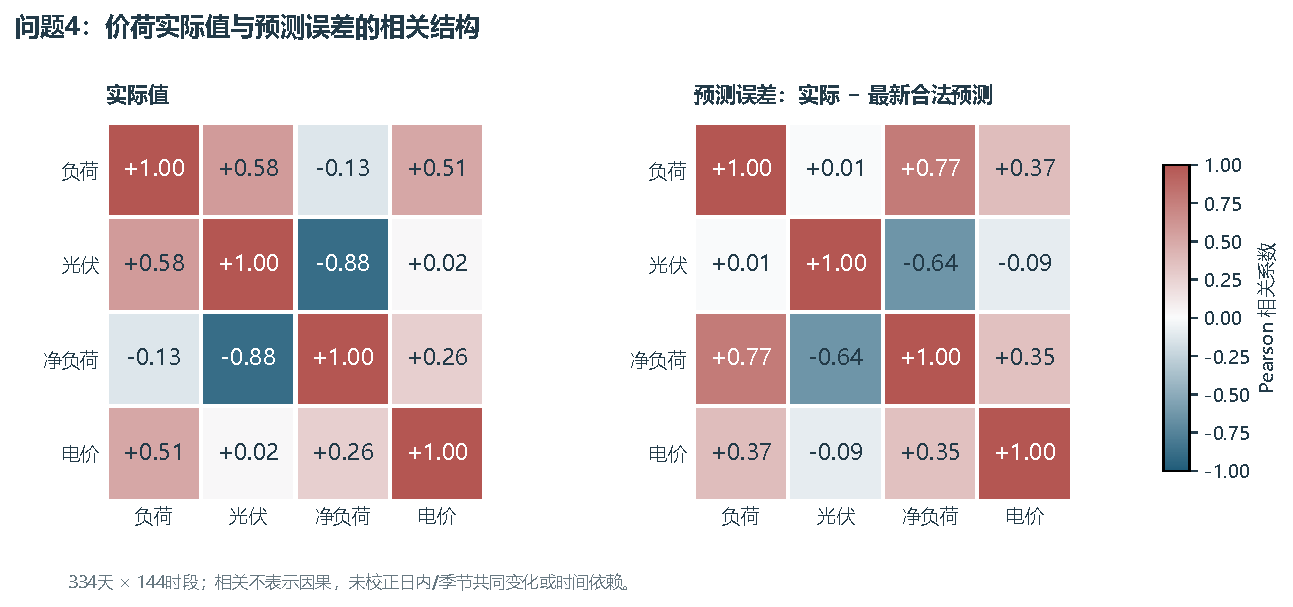
\includegraphics[width=0.91\linewidth]{figures/results/q4_correlation_heatmap.pdf}
\caption{问题四滚动配置下48096个评价时段的Pearson相关矩阵，变量依次为负荷、光伏、净负荷、电价。左图为实际值，右图为实际值减各时段最近合法预测的误差，按0、6、12、18时各覆盖36段拼接；色标为$-1$至1。矩阵仅作事后描述，不用于选型或构造当天未来场景，未作时序相关校正或因果推断。}
\label{fig:q4-correlation}
\end{figure}

\subsubsection{动态日前采购与动态滚动采购的共同优化结构}

在每个外层时点，记$\bar p_t=\sum_s\pi_sp_{t,s}$，共享参考储能仍为$c_t,d_t,e_{t+1}$，紧急补购为$h_{t,s}$。动态日前案在零时求解
\begin{equation}
 \min\left\{\sum_{t=0}^{143}\bar p_tg_t+
  \sum_s\pi_s\sum_{t=0}^{143}5p_{t,s}h_{t,s}
  +\beta_T|e_{144}-6000|\right\},
 \label{eq:q4_day_ahead_objective}
\end{equation}
满足式\eqref{eq:scenario_balance}及储能物理约束，初态取当日实际承接库存。该模型的常规采购按场景均价评价，紧急费用则逐场景乘对应价格，因此保留了高缺口与高价同时出现时的损失。

动态滚动母模型的零时模型同式\eqref{eq:q4_day_ahead_objective}，在6、12、18时采用式\eqref{eq:q3_revision_objective}--\eqref{eq:q3_revision_contract}，把固定电价替换为本次联合场景价格。最终滚动案在四个合法时点均将该LP作为一个购电候选，与点预测、三个误差余量以及日内当前合同候选按式\eqref{eq:q3_candidate_score}统一筛选。每次回放完整保留式\eqref{eq:joint_scenario}中同一历史日的价格--净负荷配对，情景$s$的紧急费用使用$5p_{t,s}h_{t,s}^{(k)}$；不能把所有情景的紧急量统一乘平均价格。常规计划费和调整费同样在各价格情景下计算，终端系数仍为情景加权价格序列的中位数，各候选共用该系数。

其当日真实费用仍按式\eqref{eq:settlement}计算，式中的$p_{D,t}$此时取附件4已经实现的交易价格。日前案$a_t=g_t$、没有调整费，滚动案仅在合法时点更新合同，原计划始终按计划量全额结算；两者均由当前实际供需驱动储能执行，并连续传递日末SOC。回放合同固定至午夜的近似边界同问题三，不包含未来尚未发布的预报或以后可能发生的合同修订。

主案继续预先设置$\lambda=0$、$\rho_t=0$。若采用内层LP候选，则当前价格使用已观测实价、未来价格使用合法预测，合同固定规则与跨日临时变量含义均沿用问题三。该扩展没有将场景独立的全天储能计划作为可执行控制，也没有因为电价波动就额外假设可以随时无成本修改采购。

\subsection{问题四求解}

\subsubsection{最终配置与实际求解步骤}

一月验证中，在已选预测配置下，动态日前案规则执行费用1042234.20元，LP候选为1052652.76元；动态滚动案规则执行为1043044.13元，剩余日LP为1057597.78元，LP加跨日为1047012.91元，详见表\ref{tab:v2_controller_validation}。该比较基于未启用候选筛选的母模型，两案据此冻结规则执行器，不根据2--12月费用重新选择执行器。零风险与零备用仍是预定经济基准，并非从验证数据中搜索出来的参数最优结论。采购筛选的适用范围与时点另依据开发期回测确定：日前版启用筛选增费0.428\%，故保留母模型；滚动版采用表\ref{tab:outer_timing_ablation}中费用最低的零时与日内均筛选配置。最终配置固定后的报告口径为开发期闭环评价。

求解时先读取该时点已发布预报和已实现历史，构造同日价荷残差场景；日前版由情景LP直接确定常规计划，滚动版由各候选LP和同规则回放确定所选合同；按当前实际净负荷执行储能、记录必要紧急补购；最后按实际价格逐项计算账单。所有未来真实负荷、光伏和价格仅在其实现后进入执行与结算，场景均价不会代替实际价格填写费用。日前案与滚动案的2月初始SOC分别为9251.54、9030.40 kWh，均来自各自固定的一月运行前缀。

\subsubsection{全年费用、紧急需求与价格不确定性的影响}

动态日前案334天计划费用14280142.03元、紧急费用513982.26元，总费用14794124.29元，紧急量80544.00 kWh，涉及106天、596个十分钟时段。最终动态滚动案计划费用14265228.71元、调整费用283142.26元、紧急费用121866.90元，总费用14670237.87元，紧急量21293.41 kWh，涉及116天、418个十分钟时段。两案总费用相差123886.42元，即滚动案低0.8374\%，紧急量低73.56\%。

图\ref{fig:q4-cost-waterfall}把日前母模型到最终滚动案的总费用变化拆成计划、调整及紧急三项：滚动案计划费用减少14913.32元、紧急费用减少392115.36元，同时新增调整费用283142.26元。三项使用未舍入数据计算，总差以完整账单为准。减少昂贵补购不必然带来同比例的总节费，额外承诺和修订仍要付款。

\begin{figure}[htbp]\centering
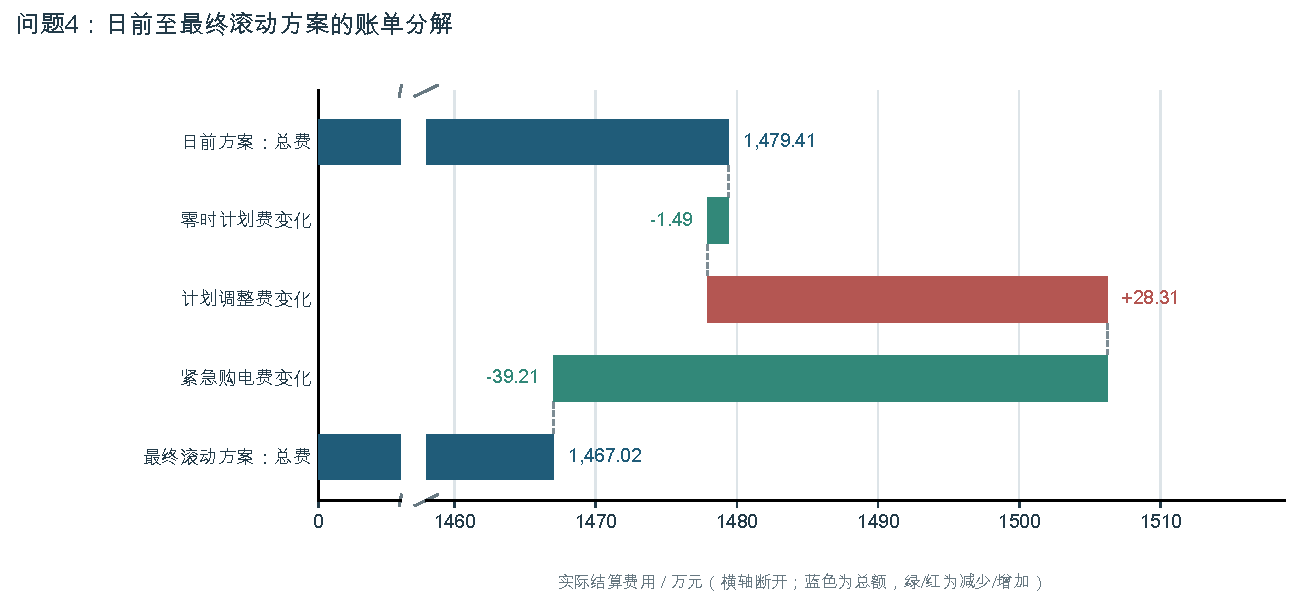
\includegraphics[width=0.95\linewidth]{figures/results/q4_cost_waterfall.pdf}
\caption{动态日前母模型到全时点筛选滚动案的实际费用分解。横轴单位为万元并明确断轴，起止条从零累计至334天总费用，中间条分别为计划费、调整费和紧急费的变化，均来自最终配置的执行结果源；两案预测配置、筛选设置与初态不同，因此这是整体策略账单差，不是单一模块的因果节费。}
\label{fig:q4-cost-waterfall}
\end{figure}

最终动态滚动案实际日总费用CVaR95为77575.87元，动态日前案为83044.31元；最高日费用分别为81797.18元和108080.37元。这里的CVaR根据334个已实现日账单计算，是描述性尾部指标，不是启用额外风险惩罚的效果证明。两案期末库存分别为6274.99与6269.86 kWh，库存差与预测、初态差异一并报告；不把账单比较称为全局最优策略间的差距。

针对筛选模块本身，应与本问未筛选的滚动母模型14769232.53元比较，而非用日前案代替同条件基线。表\ref{tab:outer_timing_ablation}与表\ref{tab:outer_screening_tradeoff}表明，全时点筛选比该基线节省98994.66元，但紧急量增加9342.73 kWh，日费用CVaR95也由77420.84元升至77575.87元。因而本次选择体现为平均账单经济性与紧急补购、尾部费用之间的权衡，不能描述为各项指标全面改善。

\subsubsection{指定日期采购、储能与紧急购电结果}

以下分别给出动态日前母模型和最终全时点筛选滚动案在四个指定日期的六个指定时段采购量、全天常规量、储能四小时汇总及紧急购电区间。购电量均为kWh，完整费用包含紧急补购；计划费用和调整费用另在分解表中列出。表格、运行轨迹及结果工作簿均由各自最终配置的执行数组生成，使用同一物理时间索引，保留原模板显示标签，不再按标签循环平移数据。

\begin{table}[htbp]\centering\small
\caption{问题4-2指定日期购电结果（沿用题目表1布局，电量单位：kWh）}
\label{tab:q4_2-purchase}
\par\smallskip\textbf{2025-03-20}\par\smallskip
\begin{tabularx}{\linewidth}{lRlRlR}
\toprule
时间段 & 购电量 & 时间段 & 购电量 & 时间段 & 购电量\\
\midrule
10:00--10:10 & 0.00 & 12:00--12:10 & 564.20 & 14:00--14:10 & 0.00\\
16:00--16:10 & 490.32 & 18:00--18:10 & 0.00 & 20:00--20:10 & 743.27\\
\midrule
全天购电量 & 67869.67 & \multicolumn{2}{c}{全天购电费（元）} & \multicolumn{2}{r}{42207.16}\\
\bottomrule
\end{tabularx}
\par\smallskip\textbf{2025-06-21}\par\smallskip
\begin{tabularx}{\linewidth}{lRlRlR}
\toprule
时间段 & 购电量 & 时间段 & 购电量 & 时间段 & 购电量\\
\midrule
10:00--10:10 & 0.00 & 12:00--12:10 & 0.00 & 14:00--14:10 & 0.00\\
16:00--16:10 & 296.43 & 18:00--18:10 & 510.07 & 20:00--20:10 & 0.00\\
\midrule
全天购电量 & 40675.72 & \multicolumn{2}{c}{全天购电费（元）} & \multicolumn{2}{r}{21012.94}\\
\bottomrule
\end{tabularx}
\par\smallskip\textbf{2025-09-23}\par\smallskip
\begin{tabularx}{\linewidth}{lRlRlR}
\toprule
时间段 & 购电量 & 时间段 & 购电量 & 时间段 & 购电量\\
\midrule
10:00--10:10 & 0.00 & 12:00--12:10 & 497.24 & 14:00--14:10 & 0.00\\
16:00--16:10 & 537.29 & 18:00--18:10 & 0.00 & 20:00--20:10 & 0.00\\
\midrule
全天购电量 & 69762.68 & \multicolumn{2}{c}{全天购电费（元）} & \multicolumn{2}{r}{48309.88}\\
\bottomrule
\end{tabularx}
\par\smallskip\textbf{2025-12-21}\par\smallskip
\begin{tabularx}{\linewidth}{lRlRlR}
\toprule
时间段 & 购电量 & 时间段 & 购电量 & 时间段 & 购电量\\
\midrule
10:00--10:10 & 0.00 & 12:00--12:10 & 970.92 & 14:00--14:10 & 0.00\\
16:00--16:10 & 851.12 & 18:00--18:10 & 744.23 & 20:00--20:10 & 0.00\\
\midrule
全天购电量 & 100945.95 & \multicolumn{2}{c}{全天购电费（元）} & \multicolumn{2}{r}{77020.40}\\
\bottomrule
\end{tabularx}
\par\smallskip\parbox{\linewidth}{\footnotesize 注：问题2与4-2列示计划购电量；问题3与4-3列示最终生效的调整后常规购电量。全天购电量不含紧急购电，全天购电费含计划、调整与紧急费用。}
\end{table}

\begin{table}[htbp]\centering\small
\caption{问题4-2指定日期储能结果（沿用题目表2布局，单位：kWh）}
\label{tab:q4_2-battery}
\par\smallskip\textbf{2025-03-20}\par\smallskip
\begin{tabularx}{\linewidth}{lRRlRR}
\toprule
时间段 & 充电量 & 放电量 & 时间段 & 充电量 & 放电量\\
\midrule
00:00--04:00 & 3824.42 & 134.84 & 04:00--08:00 & 1669.83 & 5857.47\\
08:00--12:00 & 6146.04 & 2777.38 & 12:00--16:00 & 3907.13 & 420.71\\
16:00--20:00 & 174.78 & 6369.00 & 20:00--24:00 & 5798.62 & 2212.03\\
\midrule
0:00储电量 & \multicolumn{2}{r}{6834.43} & 24:00储电量 & \multicolumn{2}{r}{6457.15}\\
\bottomrule
\end{tabularx}
\par\smallskip\textbf{2025-06-21}\par\smallskip
\begin{tabularx}{\linewidth}{lRRlRR}
\toprule
时间段 & 充电量 & 放电量 & 时间段 & 充电量 & 放电量\\
\midrule
00:00--04:00 & 963.51 & 3780.66 & 04:00--08:00 & 1400.69 & 1719.95\\
08:00--12:00 & 6932.04 & 0.00 & 12:00--16:00 & 0.00 & 0.00\\
16:00--20:00 & 0.00 & 4853.45 & 20:00--24:00 & 7501.98 & 3091.92\\
\midrule
0:00储电量 & \multicolumn{2}{r}{8545.17} & 24:00储电量 & \multicolumn{2}{r}{8723.59}\\
\bottomrule
\end{tabularx}
\par\smallskip\textbf{2025-09-23}\par\smallskip
\begin{tabularx}{\linewidth}{lRRlRR}
\toprule
时间段 & 充电量 & 放电量 & 时间段 & 充电量 & 放电量\\
\midrule
00:00--04:00 & 5330.27 & 22.20 & 04:00--08:00 & 206.94 & 5820.07\\
08:00--12:00 & 5946.19 & 1896.62 & 12:00--16:00 & 3587.87 & 530.87\\
16:00--20:00 & 163.52 & 6562.31 & 20:00--24:00 & 5525.15 & 1842.66\\
\midrule
0:00储电量 & \multicolumn{2}{r}{6002.76} & 24:00储电量 & \multicolumn{2}{r}{6159.23}\\
\bottomrule
\end{tabularx}
\par\smallskip\textbf{2025-12-21}\par\smallskip
\begin{tabularx}{\linewidth}{lRRlRR}
\toprule
时间段 & 充电量 & 放电量 & 时间段 & 充电量 & 放电量\\
\midrule
00:00--04:00 & 4499.29 & 40.16 & 04:00--08:00 & 0.00 & 741.76\\
08:00--12:00 & 5940.70 & 6486.91 & 12:00--16:00 & 5724.46 & 2220.11\\
16:00--20:00 & 0.00 & 5500.96 & 20:00--24:00 & 5818.48 & 2842.53\\
\midrule
0:00储电量 & \multicolumn{2}{r}{6795.26} & 24:00储电量 & \multicolumn{2}{r}{6766.10}\\
\bottomrule
\end{tabularx}
\end{table}

\begin{table}[htbp]\centering\small
\caption{问题4-2指定日期紧急购电（题目表3布局，单位：kWh）}
\label{tab:q4_2-emergency}
\setlength{\tabcolsep}{3pt}
\begin{tabularx}{\linewidth}{lRlRlRlR}\toprule
\multicolumn{2}{c}{2025-03-20} & \multicolumn{2}{c}{2025-06-21} & \multicolumn{2}{c}{2025-09-23} & \multicolumn{2}{c}{2025-12-21}\\
时间段 & 购电量 & 时间段 & 购电量 & 时间段 & 购电量 & 时间段 & 购电量\\\midrule
无 & 0.00 & 无 & 0.00 & 18:20--18:40 & 3.91 & 无 & 0.00\\
 &   &  &   & 20:30--20:40 & 357.19 &  &  \\
 &   &  &   & 20:50--21:10 & 90.05 &  &  \\
 &   &  &   & 21:20--21:50 & 34.20 &  &  \\
\midrule
合计 & 0.00 & 合计 & 0.00 & 合计 & 485.35 & 合计 & 0.00\\
\bottomrule\end{tabularx}\end{table}
\begin{table}[htbp]\centering\small
\caption{问题4-2指定日期计划、调整与费用分解}
\begin{tabularx}{\linewidth}{lRRRRR}\toprule
日期 & 计划量/kWh & 生效量/kWh & 计划费/元 & 调整费/元 & 紧急费/元\\\midrule
2025-03-20 & 67869.67 & 67869.67 & 42207.16 & 0.00 & 0.00\\
2025-06-21 & 40675.72 & 40675.72 & 21012.94 & 0.00 & 0.00\\
2025-09-23 & 69762.68 & 69762.68 & 45194.04 & 0.00 & 3115.84\\
2025-12-21 & 100945.95 & 100945.95 & 77020.40 & 0.00 & 0.00\\
\bottomrule\end{tabularx}\end{table}
\FloatBarrier
\begin{table}[htbp]\centering\small
\caption{问题4-3指定日期购电结果（沿用题目表1布局，电量单位：kWh）}
\label{tab:q4_3-purchase}
\par\smallskip\textbf{2025-03-20}\par\smallskip
\begin{tabularx}{\linewidth}{lRlRlR}
\toprule
时间段 & 购电量 & 时间段 & 购电量 & 时间段 & 购电量\\
\midrule
10:00--10:10 & 0.00 & 12:00--12:10 & 624.29 & 14:00--14:10 & 0.00\\
16:00--16:10 & 671.04 & 18:00--18:10 & 704.20 & 20:00--20:10 & 743.27\\
\midrule
全天购电量 & 71574.04 & \multicolumn{2}{c}{全天购电费（元）} & \multicolumn{2}{r}{45107.31}\\
\bottomrule
\end{tabularx}
\par\smallskip\textbf{2025-06-21}\par\smallskip
\begin{tabularx}{\linewidth}{lRlRlR}
\toprule
时间段 & 购电量 & 时间段 & 购电量 & 时间段 & 购电量\\
\midrule
10:00--10:10 & 0.00 & 12:00--12:10 & 0.00 & 14:00--14:10 & 0.00\\
16:00--16:10 & 260.52 & 18:00--18:10 & 495.32 & 20:00--20:10 & 0.00\\
\midrule
全天购电量 & 37518.90 & \multicolumn{2}{c}{全天购电费（元）} & \multicolumn{2}{r}{19308.93}\\
\bottomrule
\end{tabularx}
\par\smallskip\textbf{2025-09-23}\par\smallskip
\begin{tabularx}{\linewidth}{lRlRlR}
\toprule
时间段 & 购电量 & 时间段 & 购电量 & 时间段 & 购电量\\
\midrule
10:00--10:10 & 22.75 & 12:00--12:10 & 461.07 & 14:00--14:10 & 54.35\\
16:00--16:10 & 611.01 & 18:00--18:10 & 0.00 & 20:00--20:10 & 822.11\\
\midrule
全天购电量 & 73431.36 & \multicolumn{2}{c}{全天购电费（元）} & \multicolumn{2}{r}{47890.72}\\
\bottomrule
\end{tabularx}
\par\smallskip\textbf{2025-12-21}\par\smallskip
\begin{tabularx}{\linewidth}{lRlRlR}
\toprule
时间段 & 购电量 & 时间段 & 购电量 & 时间段 & 购电量\\
\midrule
10:00--10:10 & 0.00 & 12:00--12:10 & 1054.19 & 14:00--14:10 & 0.00\\
16:00--16:10 & 877.48 & 18:00--18:10 & 744.23 & 20:00--20:10 & 0.00\\
\midrule
全天购电量 & 101918.89 & \multicolumn{2}{c}{全天购电费（元）} & \multicolumn{2}{r}{77624.69}\\
\bottomrule
\end{tabularx}
\par\smallskip\parbox{\linewidth}{\footnotesize 注：问题2与4-2列示计划购电量；问题3与4-3列示最终生效的调整后常规购电量。全天购电量不含紧急购电，全天购电费含计划、调整与紧急费用。}
\end{table}

\begin{table}[htbp]\centering\small
\caption{问题4-3指定日期储能结果（沿用题目表2布局，单位：kWh）}
\label{tab:q4_3-battery}
\par\smallskip\textbf{2025-03-20}\par\smallskip
\begin{tabularx}{\linewidth}{lRRlRR}
\toprule
时间段 & 充电量 & 放电量 & 时间段 & 充电量 & 放电量\\
\midrule
00:00--04:00 & 4119.21 & 134.84 & 04:00--08:00 & 825.23 & 5868.37\\
08:00--12:00 & 5765.88 & 2777.38 & 12:00--16:00 & 5187.95 & 254.72\\
16:00--20:00 & 28.20 & 6553.40 & 20:00--24:00 & 5792.33 & 1970.23\\
\midrule
0:00储电量 & \multicolumn{2}{r}{6530.78} & 24:00储电量 & \multicolumn{2}{r}{6567.77}\\
\bottomrule
\end{tabularx}
\par\smallskip\textbf{2025-06-21}\par\smallskip
\begin{tabularx}{\linewidth}{lRRlRR}
\toprule
时间段 & 充电量 & 放电量 & 时间段 & 充电量 & 放电量\\
\midrule
00:00--04:00 & 675.55 & 4135.87 & 04:00--08:00 & 1424.39 & 1719.95\\
08:00--12:00 & 8481.89 & 0.00 & 12:00--16:00 & 0.00 & 0.00\\
16:00--20:00 & 0.00 & 5210.22 & 20:00--24:00 & 6461.65 & 2485.90\\
\midrule
0:00储电量 & \multicolumn{2}{r}{7782.84} & 24:00储电量 & \multicolumn{2}{r}{8064.24}\\
\bottomrule
\end{tabularx}
\par\smallskip\textbf{2025-09-23}\par\smallskip
\begin{tabularx}{\linewidth}{lRRlRR}
\toprule
时间段 & 充电量 & 放电量 & 时间段 & 充电量 & 放电量\\
\midrule
00:00--04:00 & 5172.38 & 22.20 & 04:00--08:00 & 177.31 & 5680.26\\
08:00--12:00 & 6536.73 & 1893.23 & 12:00--16:00 & 3099.44 & 353.23\\
16:00--20:00 & 96.08 & 6443.21 & 20:00--24:00 & 5603.57 & 2259.51\\
\midrule
0:00储电量 & \multicolumn{2}{r}{6144.86} & 24:00储电量 & \multicolumn{2}{r}{6260.00}\\
\bottomrule
\end{tabularx}
\par\smallskip\textbf{2025-12-21}\par\smallskip
\begin{tabularx}{\linewidth}{lRRlRR}
\toprule
时间段 & 充电量 & 放电量 & 时间段 & 充电量 & 放电量\\
\midrule
00:00--04:00 & 4436.14 & 40.16 & 04:00--08:00 & 735.70 & 1384.74\\
08:00--12:00 & 6412.06 & 6391.52 & 12:00--16:00 & 5218.63 & 2240.52\\
16:00--20:00 & 0.00 & 5490.42 & 20:00--24:00 & 5769.36 & 2842.53\\
\midrule
0:00储电量 & \multicolumn{2}{r}{6852.09} & 24:00储电量 & \multicolumn{2}{r}{6733.60}\\
\bottomrule
\end{tabularx}
\end{table}

\begin{table}[htbp]\centering\small
\caption{问题4-3指定日期紧急购电（题目表3布局，单位：kWh）}
\label{tab:q4_3-emergency}
\setlength{\tabcolsep}{3pt}
\begin{tabularx}{\linewidth}{lRlRlRlR}\toprule
\multicolumn{2}{c}{2025-03-20} & \multicolumn{2}{c}{2025-06-21} & \multicolumn{2}{c}{2025-09-23} & \multicolumn{2}{c}{2025-12-21}\\
时间段 & 购电量 & 时间段 & 购电量 & 时间段 & 购电量 & 时间段 & 购电量\\\midrule
无 & 0.00 & 无 & 0.00 & 18:30--18:40 & 2.38 & 无 & 0.00\\
 &   &  &   & 20:10--20:20 & 10.23 &  &  \\
\midrule
合计 & 0.00 & 合计 & 0.00 & 合计 & 12.61 & 合计 & 0.00\\
\bottomrule\end{tabularx}\end{table}
\begin{table}[htbp]\centering\small
\caption{问题4-3指定日期计划、调整与费用分解}
\begin{tabularx}{\linewidth}{lRRRRR}\toprule
日期 & 计划量/kWh & 生效量/kWh & 计划费/元 & 调整费/元 & 紧急费/元\\\midrule
2025-03-20 & 71574.04 & 71574.04 & 45107.31 & 0.00 & 0.00\\
2025-06-21 & 37505.63 & 37518.90 & 19288.01 & 20.91 & 0.00\\
2025-09-23 & 73403.01 & 73431.36 & 47750.49 & 57.78 & 82.45\\
2025-12-21 & 101918.89 & 101918.89 & 77624.69 & 0.00 & 0.00\\
\bottomrule\end{tabularx}\end{table}
\FloatBarrier

\subsubsection{跨月份表现与模型适用边界}

图\ref{fig:v2-monthly}将四组最终配置的实际费用与紧急量按月汇总：问题二与第四问日前版保留母模型，问题三与第四问滚动版采用全时点筛选。月度波动同时包含季节负荷、光伏、价格及历史误差变化，不能仅凭某月曲线把差异归因于价格预测。联合场景通过同日配对保持数据中已存在的价荷关系，但28个历史日仍可能遗漏稀少高价缺口，也不能据此保证跨年份泛化。

\begin{figure}[htbp]\centering
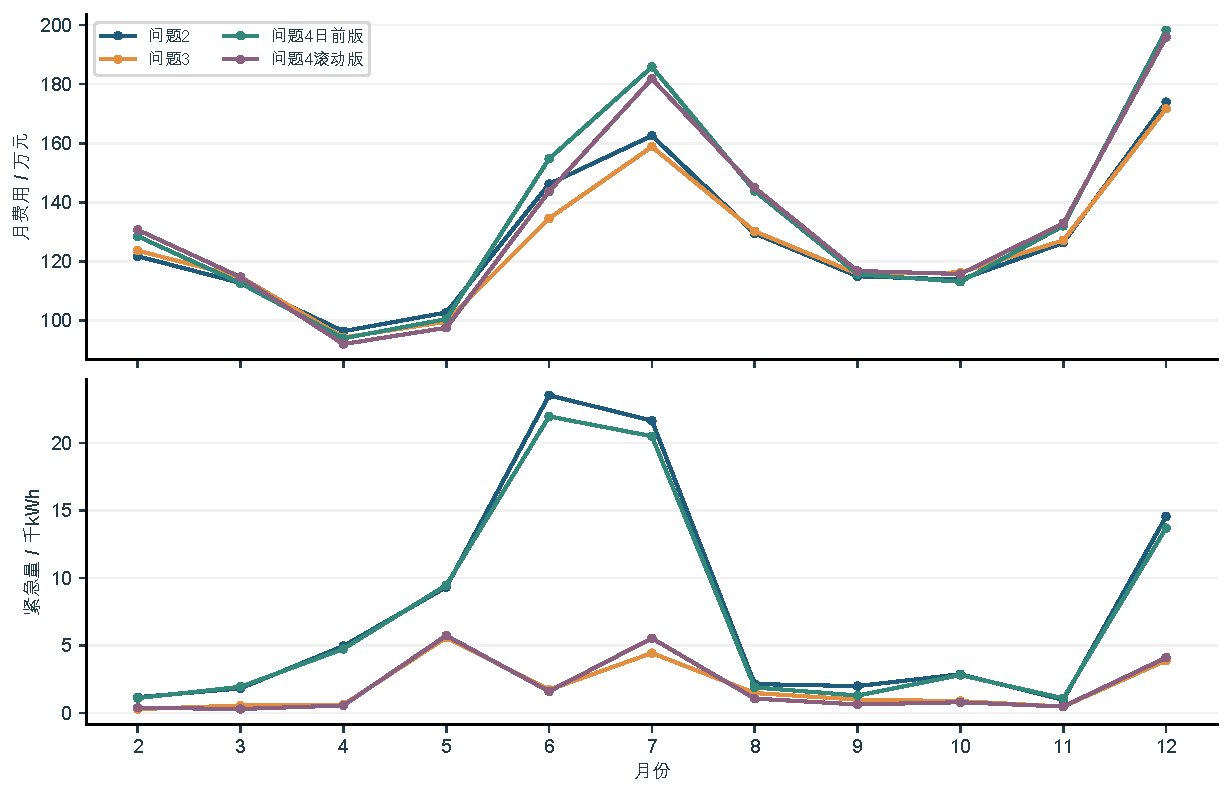
\includegraphics[width=0.95\linewidth]{figures/results/v2_monthly.pdf}
\caption{问题二至四四组最终配置的月度实际费用与紧急购电量。日前两组采用母模型，滚动两组采用全时点筛选；每月数值由2--12月逐日执行账单和电量求和，非优化器辅助目标，不同方案的预测来源、筛选设置与初态差异需结合正文解释。}
\label{fig:v2-monthly}
\end{figure}

本问的机制结论是：未知价格使场景的经济权重随价格改变，故采购应联合考虑价荷而非只拟合需求均值；储能和滚动修订再处理跨时段与信息更新。配对情景下的同规则候选回放支持在本次开发期为滚动版采用全时点筛选，但日前版没有获益，紧急补购和尾部费用也可能增加。严格多阶段非预见性、未来修订机会的显式价值与完整跨日随机结算仍属于未实现的增强，不能将当前有限候选的费用最低结论推广为未来全局最优保证。
\FloatBarrier
